
%(BEGIN_QUESTION)
% Copyright 2015, Tony R. Kuphaldt, released under the Creative Commons Attribution License (v 1.0)
% This means you may do almost anything with this work of mine, so long as you give me proper credit

\noindent
{\bf Lab Exercise}

\vskip 5pt

Your task is to build, document, and successfully operate a process controlled by a recording PID controller.  Several alternative process types exist and are documented in subsequent pages.  The working process you build will be used in future lab exercises this quarter to meet other learning objectives, which means you will {\it not} disassemble this project at the completion of these lab objectives as you normally would.

The following table of objectives show what you and your team must complete within the scheduled time for this lab exercise.  Note how some of these objectives are individual, while others are for the team as a whole:

\underbar{Objective completion table:}

% No blank lines allowed between lines of an \halign structure!
% I use comments (%) instead, so that TeX doesn't choke.

$$\vbox{\offinterlineskip
\halign{\strut
\vrule \quad\hfil # \ \hfil & 
\vrule \quad\hfil # \ \hfil & 
\vrule \quad\hfil # \ \hfil & 
\vrule \quad\hfil # \ \hfil & 
\vrule \quad\hfil # \ \hfil & 
\vrule \quad\hfil # \ \hfil & 
\vrule \quad\hfil # \ \hfil \vrule \cr
\noalign{\hrule}
%
% First row
{\bf Performance objective} & {\bf Grading} & {\bf 1} & {\bf 2} & {\bf 3} & {\bf 4} & {\bf Team} \cr
%
\noalign{\hrule}
%
% Another row
Choose process to build & mastery & -- & -- & -- & -- & \cr
%
\noalign{\hrule}
%
% Another row
Team meeting and prototype sketch & mastery & -- & -- & -- & -- & \cr
%
\noalign{\hrule}
%
% Another row
Circuit design challenge & mastery & & & & & -- -- -- -- \cr
%
\noalign{\hrule}
%
% Another row
Final loop diagram and system inspection & mastery & & & & & -- -- -- -- \cr
%
\noalign{\hrule}
%
% Another row
Process and Instrument Diagram (P\&ID) & mastery & & & & & -- -- -- -- \cr
%
\noalign{\hrule}
%
% Another row
Trend graph displays PV and Output & mastery & -- & -- & -- & -- &  \cr
%
\noalign{\hrule}
%
% Another row
Process exhibits good control behavior & mastery & -- & -- & -- & -- &  \cr
%
\noalign{\hrule}
%
% Another row
PV alarm(s) defined and enabled & mastery & -- & -- & -- & -- &  \cr
%
\noalign{\hrule}
%
% Another row
Lab question: Instrument connections & proportional &  &  &  &  & -- -- -- -- \cr
%
\noalign{\hrule}
%
% Another row
Lab question: Commissioning & proportional &  &  &  &  & -- -- -- -- \cr
%
\noalign{\hrule}
%
% Another row
Lab question: Mental math & proportional &  &  &  &  & -- -- -- -- \cr
%
\noalign{\hrule}
%
% Another row
Lab question: Diagnostics & proportional &  &  &  &  & -- -- -- -- \cr
%
\noalign{\hrule}
} % End of \halign 
}$$ % End of \vbox

The only ``proportional'' scoring in this activity are the lab questions, which are answered by each student individually.  A listing of potential lab questions are shown at the end of this worksheet question.  The lab questions are intended to guide your labwork as much as they are intended to measure your comprehension, and as such the instructor may ask these questions of your team day by day, rather than all at once (on a single day).

\vskip 10pt

{\bf It is essential that your team plans ahead what to accomplish each day.  A short (10 minute) team meeting at the beginning of each lab session is a good way to do this, reviewing what's already been done, what's left to do, and what assessments you should be ready for.  There is a lot of work involved with building, documenting, and troubleshooting these working instrument systems!}

As you and your team work on this system, you will invariably encounter problems.  You should always attempt to solve these problems as a team before requesting instructor assistance.  If you still require instructor assistance, write your team's color on the lab whiteboard with a brief description of what you need help on.  The instructor will meet with each team in order they appear on the whiteboard to address these problems.

$$\includegraphics[width=15.5cm]{i01558x01.eps}$$





\vfil \eject

\noindent
{\bf Lab Exercise -- choosing a process to build}

\vskip 5pt

There are a number of process types to choose from when selecting the one you will build with your team.  The only non-negotiable limitations is that the process must be safe, legal, and possible to complete in the time allotted for this lab.  What follows are some examples:

$$\includegraphics[width=15.5cm]{i01558x02.eps}$$

$$\includegraphics[width=15.5cm]{i01558x03.eps}$$

\filbreak

$$\includegraphics[width=15.5cm]{i01558x04.eps}$$

$$\includegraphics[width=15.5cm]{i01558x05.eps}$$

\filbreak

$$\includegraphics[width=15.5cm]{i01558x06.eps}$$

$$\includegraphics[width=15.5cm]{i01558x07.eps}$$

\noindent
Other process ideas include:

\begin{itemize}
\item{} Soldering iron temperature control (blowing air over tip with variable-speed fan).
\vskip 10pt
\item{} Draft pressure control (controlling very low air pressure inside of a box). 
\vskip 10pt
\item{} Pneumatic piston height control (using lengths of PVC pipe to build a simple piston/cylinder which may be used to lift small weights using modest air pressures).  A good way to control air pressure to the piston is to route the I/P transducer's output to a {\it volume booster} relay and let the relay's output directly drive the piston.  Piston height may be sensed using a flexible water tube attached to the piston rod, running to a stationary pressure transmitter.
\vskip 10pt
\item{} Sterno-fired air heat exchanger. 
\vskip 10pt
\item{} Miniature steam boiler.  {\it Note: this is an advanced project!}
\vskip 10pt
\item{} Air/Fuel ratio burner control.  {\it Note: this is an advanced project!}
\vskip 10pt
\item{} Servomechanism position control.  {\it Note: this is an advanced project!}
\vskip 10pt
\item{} Inverted pendulum balance.  {\it Note: this is a \underbar{very} advanced project!}
\end{itemize}






\vfil \eject

\noindent
{\bf Lab Exercise -- team meeting, prototype sketch, and instrument selection}

\vskip 5pt

An important first step in completing this lab exercise is to {\bf meet with your instructor} as a team to discuss safety concerns, team performance, and specific roles for team members.  If you would like to emphasize exposure to certain equipment (e.g. use a particular type of control system, certain power tools), techniques (e.g. fabrication), or tasks to improve your skill set, this is the time to make requests of your team so that your learning during this project will be maximized.

\vskip 10pt

An absolutely essential step in completing this lab exercise is to work together as a team to {\bf sketch a prototype diagram} showing what you intend to build.  This usually takes the form of a simple electrical schematic and/or loop diagram showing all electrical connections between components, as well as any tubing or piping for fluids.  This prototype sketch need not be exhaustive in detail, but it does need to show enough detail for the instructor to determine if all components will be correctly connected for their safe function.

For example, if you intend to connect field devices to a PLC (Programmable Logic Controller), your prototype sketch must show how those devices will connect to typical input/output terminals on the PLC, where electrical power will be supplied, etc.  Prototype sketches need not show all intermediary connections between components, such as terminal blocks in junction boxes between the field device and the controller.

You should practice good problem-solving techniques when creating your prototype sketch, such as consulting equipment manuals for information on component functions and marking directions of electric current, voltage polarities, and identifying electrical sources/loads.  Use this task as an opportunity to strengthen your analytical skills!  Remember that you will be challenged in this program to do all of this on your own (during ``capstone'' assessments), so do not make the mistake of relying on your teammates to figure this out for you -- instead, treat this as a problem {\it you} must solve and compare your results with those of your teammates.

Your team's prototype sketch is so important that the instructor will demand you provide this plan before any construction on your team's working system begins.  {\it Any team found constructing their system without a verified plan will be ordered to cease construction and not resume until a prototype plan has been drafted and approved!}  Similarly, you should not deviate from the prototype design without instructor approval, to ensure nothing will be done to harm equipment by way of incorrect connections.  Each member on the team should have ready access to this plan (ideally possessing their own copy of the plan) throughout the construction process.  Prototype design sketching is a skill and a habit you should cultivate in school and take with you in your new career.

\vskip 10pt

When selecting field instruments for this lab exercise, choose a {\it transmitter} suitable for measuring your process variable, and likely an {\it I/P converter} used to convert the controller's 4-20 mA output signal into an air pressure that a control valve may operate on.  Electronic process controllers are in several locations throughout the lab, ready to be used for controlling processes.  Your instructor will help you select appropriate instruments for the process you have chosen.

You may also need a {\it data acquisition unit}, or {\it DAQ} to function as a trend recorder.  When used with a personal computer and connected properly to the loop circuit, a DAQ unit will provide graphical displays of loop variables over time.  Students usually find the connection of a DAQ unit to their loop controller to be the trickiest part of their loop wiring.  You will need to consult the manufacturer documentation on the DAQ unit as well as the field instruments and controller in order to figure out how to wire them together.  Even if your process controller already provides trending capability, you may find connection of a DAQ unit to your loop circuits a useful exercise because the ability to quickly connect and use DAQ hardware and software to monitor electrical parameters in a system is a valuable diagnostic skill in this career.

You will find your teammates who have already taken the Measurement course series (INST24X) will be very helpful in showing you how to check, configure, calibrate, and install the measuring instrument(s) you will need for your process!

\vskip 10pt

{\bf Planning a functioning system should take no more than an hour if the team is working efficiently, and will save you hours of frustration (and possible component destruction!).}






\vfil \eject

\noindent
{\bf Lab Exercise -- circuit design challenge}

\vskip 5pt

Your instructor will choose one 4-20 mA field instrument and one control system from the lists shown below, for which you must sketch an accurate circuit diagram showing how the two instruments would connect to each other.  If this interconnection between controller and field instrument requires additional electrical components to function (e.g. DC or AC power source, precision 250 $\Omega$ resistor, diode, relay, etc.), those must be incorporated into your diagram as well.  Instruction manuals for all instrument listed are available on the electronic Instrumentation Reference for your convenience.  When your sketch is complete, you must show the relevant manual pages to your instructor for verification of correct connections.

This exercise tests your ability to locate appropriate information in technical manuals and design a correct 4-20 mA analog signal circuit for a given pair of instruments.  The electronic Instrumentation Reference will be available to you in order to answer this question.

\vskip 10pt

Since all 4-20 mA ``loops'' are basically series DC circuits, it is highly recommended that you approach their design the same as for any other DC circuit: carefully identify all {\it sources} and {\it loads} in the circuit, trace directions of all currents, and mark the polarities of all voltages.  Most of the mistakes made in this type of circuit design challenge may be remedied by careful consideration of these specific circuit-analysis details.

%%%%%%%%%%%%%%%%%%%%%%%%%%%%%%%
\vskip 10pt
\filbreak
\hbox{ \vrule
\vbox{ \hrule \vskip 3pt
\hbox{ \hskip 3pt
\vbox{ \hsize=5in \raggedright

\noindent \centerline{\bf 4-20 mA transmitter options}
\begin{itemize}
\item{} Pressure

	\begin{itemize}
	\item{} Yokogawa DPharp EJX110A or EJX910 
	\item{} Honeywell ST3000
	\end{itemize}
\vskip 2pt
\item{} Level
\vskip 2pt

\item{} Temperature
		\begin{itemize}
		\item{} Foxboro RTT15 or RTT30
		\item{} Moore Industries SPT with sourcing (4-wire) 4-20 mA output
		\item{} Moore Industries SPT with sinking (2-wire) 4-20 mA output
		\item{} Moore Industries TRX or TDY
		%\item{} Honeywell STT173
		\end{itemize}
\vskip 2pt
\item{} Flow

\vskip 2pt
\item{} Analytical
	\begin{itemize}
	\item{} Daniel 700 gas chromatograph (4 analog output channels)
	\item{} Foxboro 876PH (pH/ORP/ISE)
	\end{itemize}
\end{itemize}

} \hskip 3pt}%
\vskip 5pt \hrule}%
\vrule}
%%%%%%%%%%%%%%%%%%%%%%%%%%%%%%%




%%%%%%%%%%%%%%%%%%%%%%%%%%%%%%%
\vskip 10pt
\filbreak
\hbox{ \vrule
\vbox{ \hrule \vskip 3pt
\hbox{ \hskip 3pt
\vbox{ \hsize=5in \raggedright

\noindent \centerline{\bf Controller options}
\begin{itemize}
\item{} Monolithic

\begin{itemize}
	\item{} Siemens 353
	\item{} Foxboro 716C
	\item{} Foxboro 718TC
	\item{} Foxboro 762CNA 
	\item{} Moore Industries 535
	\item{} Honeywell UDC2300
	\item{} Honeywell UDC3500 
\end{itemize}
\vskip 2pt
\item{} Modular -- {\it you choose the appropriate I/O module}
\begin{itemize}

	\item{} Emerson ROC800 SCADA/RTU 
\end{itemize}
\vskip 2pt
\item{} Distributed Control System (DCS) -- {\it you choose the appropriate I/O module}
\begin{itemize}

	\item{} Emerson DeltaV with S-series I/O 
	\item{} Honeywell Experion with 2MLF series I/O 
\end{itemize}
\vskip 2pt
\item{} Programmable Logic Controller (PLC) -- {\it you choose the appropriate I/O module}
\begin{itemize}

	\item{} Rockwell ControlLogix (catalog number 1756)
	\item{} Rockwell CompactLogix (catalog number 1769)
\end{itemize}

\end{itemize}

} \hskip 3pt}%
\vskip 5pt \hrule}%
\vrule}
%%%%%%%%%%%%%%%%%%%%%%%%%%%%%%%




%%%%%%%%%%%%%%%%%%%%%%%%%%%%%%%
\vskip 10pt
\filbreak
\hbox{ \vrule
\vbox{ \hrule \vskip 3pt
\hbox{ \hskip 3pt
\vbox{ \hsize=5in \raggedright

\noindent \centerline{\bf 4-20 mA Final Control Element options}
\begin{itemize}
\item{} Pneumatic control valve positioners
\begin{itemize}

\item{} Fisher DVC6000 positioner 
\end{itemize}
\vskip 2pt
\item{} Electrically actuated valves (MOV)
\begin{itemize}

\item{} Rotork AQ with Folomatic controller 
\end{itemize}
\vskip 2pt
\item{} AC motor drives (VFD)
\begin{itemize}

\item{} Automation Direct GS1 
\end{itemize}
\end{itemize}

} \hskip 3pt}%
\vskip 5pt \hrule}%
\vrule}
%%%%%%%%%%%%%%%%%%%%%%%%%%%%%%%


\vfil

Study reference: the ``Analog Electronic Instrumentation'' chapter of {\it Lessons In Industrial Instrumentation}, particularly the section on HART.

\vskip 10pt

Note: a very effective problem-solving strategy for determining how to connect different components together to create a working 4-20 mA current loop is to first identify whether each component acts as a {\it source} or a {\it load} in that loop circuit.  Then, label voltage polarities (+ , $-$) and directions of current accordingly.  Knowing which way current must flow through each component and which polarity each voltage must have is key to ensuring the inter-component connections are correct.








\vfil \eject

\noindent
{\bf Lab Exercise -- building the system}

\vskip 5pt

The Instrumentation lab is set up to facilitate the construction of working instrument ``loops,'' with over a dozen junction boxes, pre-pulled signal cables, and ``racks'' set up with 2-inch vertical pipes for mounting instruments.  These racks also provide structure for building physical processes, with more than enough weight-bearing capacity to hold any process vessels and equipment.  The only wires you should need to install to build a working system are those connecting the field instrument to the nearest junction box, and then small ``jumper'' cables connecting different pre-installed cables together within intermediate junction boxes.

After getting your prototype sketch approved by the instructor, you are cleared to begin building your system.  Instruments attach to 2-inch pipes using special brackets and U-bolts.  These brackets and U-bolts are located in the instrument storage area.  

Select a specific loop controller for your system.  Your instructor may choose the controller for your team, to ensure you learn more than one type of controller during the course of a quarter.

Finally, your process control system needs to have a loop number, so all instruments may be properly labeled.  This loop number needs to be unique, so that another team does not label their instruments and cables the same as yours.  One way to make your loop number unique is to use the equivalent resistor color-code value for your team's color in the loop number.  For example, if you are the ``Red'' team, your loop number could be ``2''. 

\vskip 10pt

{\bf Common mistakes:}

\begin{itemize}
\item{} Neglecting to consult the manufacturer's documentation for field instruments (e.g. how to wire them, how to calibrate them).
\item{} Mounting the field instrument(s) in awkward positions, making it difficult to reach connection terminals or to remove covers when installed.
\item{} Improper pipe/tube fitting installation (e.g. trying to thread tube fittings into pipe fittings and vice-versa).
\item{} Failing to tug on each and every wire where it terminates to ensure a mechanically sound connection.
\item{} Students working on portions of the system in isolation, not sharing with their teammates what they did and how.  It is important that the whole team learns all aspects of their system!
\end{itemize}

\vskip 10pt

{\bf Building a functioning process complete with instrumentation for control typically takes one or two sessions (3 hours each) if all components are readily available and the team is working efficiently!}





\vfil \eject

\noindent
{\bf Lab Exercise -- documenting the system}

\vskip 5pt

Each student must sketch their own {\it loop diagram} and their own {\it P\&ID} for their team's system, following proper ISA conventions.  The P\&ID documents the flow of fluid and materials in your process plus the general control strategy.  The loop diagram documents all wiring and tube connections between instruments.  Although the two diagrams reinforce one another and might possibly be combined into one, the industry standard is to use two separate diagrams.

Sample loop diagrams are shown in the next question in this worksheet.  These loop diagrams must be {\it comprehensive} and {\it detailed}, showing every wire connection, every cable, every terminal block, range points, etc.  The principle to keep in mind here is to make the loop diagram so complete and unambiguous that anyone can follow it to see what connects to what, even someone unfamiliar with industrial instrumentation.  In industry, loops are often constructed by contract personnel with limited understanding of how the system is supposed to function.  The loop diagrams they follow must be so complete that they will be able to connect everything properly without necessarily understanding how it is supposed to work.

Every instrument and every signal cable in your loop needs to be properly labeled with an ISA-standard tag number.  An easy way to do this is to wrap a short piece of masking tape around each cable (and placed on each instrument) then writing on that masking tape with a permanent marker.  Although no industry standard exists for labeling signal cables, a good recommendation is to label each two-wire cable with the tag number of the field instrument it goes to.  Thus, every length of two-wire cable in a pressure transmitter circuit should be labeled ``PT-$x$'' (where ``$x$'' is the loop number), every flow control valve should be labeled ``FV-$x$'', etc.  Remember that the entire loop is defined by the process variable it measures: if the PV is {\it temperature} then the transmitter with be a {\it T}T, the control valve will be a {\it T}V, the controller with be a {\it T}C, etc.

When your entire team is finished drafting your individual loop diagrams, call the instructor to do an inspection of the loop.  Here, the instructor will have students take turns going through the entire loop, with the other students checking their diagrams for errors and omissions along the way.  During this time the instructor will also inspect the quality of the installation, identifying problems such as frayed wires, improperly crimped terminals, poor cable routing, missing labels, lack of wire duct covers, etc.  The team must correct all identified errors in order to receive credit for their system.  

After successfully passing the inspection, each team member needs to place their loop diagram in the diagram holder located in the middle of the lab behind the main control panel.  When it comes time to troubleshoot another team's system, this is where you will go to find a loop diagram for that system!

The P\&ID's will be submitted to the instructor for inspection as well, but the process itself need not be inspected again.

\vskip 10pt

{\bf Common mistakes:}

\begin{itemize}
\item{} Forgetting to label all signal wires (see example loop diagrams).
\item{} Forgetting to label all field instruments with their own tag names (e.g. PT-83).
\item{} Forgetting to note all wire colors.
\item{} Forgetting to put your name on the loop diagram!
\item{} Using non-standard tags for instruments rather than ISA 5.1 standard notation.
\item{} Basing your diagram off of a team-mate's diagram, rather than closely inspecting the system for yourself.
\item{} Not placing loop sheet instruments in the correct orientation (field instruments on the left, control room instruments on the right).
\end{itemize}

\vskip 10pt

{\bf Creating and inspecting accurate loop diagrams should take no more than one full lab session (3 hours) if the team is working efficiently!  Creating and inspecting accurate P\&IDs will take more time, but not an entire lab session (3 hours).}







\vfil \eject

\noindent
{\bf Lab Exercise -- operating the system}

\vskip 5pt

All networked loop controllers in the lab (DCS, DDC, PLC, single-loop networked) provide graphing functionality so that you may plot your process variable (PV) and output values over time.  This graphical data is essential for tuning PID-controlled loops.  If you happen to be using a controller that does not provide graphing capability, your team must attach a trend recorder and/or a data acquisition unit (plus a personal computer) to the necessary signal cables so that these values are recorded over time.

PID tuning is a subject worthy of its own course, and so you will not be expected to achieve perfect control on your process.  You will find, however, that one of the best ways to learn PID tuning is by ``playing'' with your process as it responds to different tuning parameters entered into the loop controller.  The expectation for ``good control behavior'' in the context of this lab exercise is for the loop to exhibit response that is no less stable following large setpoint changes than the classic ``quarter-wave damping'' described by Ziegler and Nichols in their 1942 paper.

\vskip 10pt

Most student-built processes are quite safe to operate.  However, if your process harbors any unique hazards (e.g. overflowing water may present a slip hazard, overheated oven may cause materials to smoke or burn), you must be aware of these hazards and limit everyones' exposure to them.  All team members for each process must be familiar with the inherent hazards of their process and how to mitigate them.  One operational step to help avoid problems is to configure the controller for {\it setpoint limits} preventing the setpoint value from being placed at ``dangerous'' values in automatic mode.  Just what these setpoint limit values should be set to varies with the process and the team's experience operating it.

As your time with the process builds, you will no doubt arrive at ideas for improving it.  Feel free to work with your team to optimize the process in any way you see fit.  The goal is to have your process as robust and ``problem-free'' as possible for other teams to use it in later coursework!

\vskip 10pt

After you have built and tuned your process, you should identify and configure alarm values for the controller's PV display.  Most controllers have PV alarm capability built in, signaling a condition of excessive or insufficient PV if those alarm points are ever tripped.  You need to set at least a high alarm on the PV so that when other teams come after you to re-tune your process, they have some ``guidepost'' showing them what PV value(s) they should not exceed!  If your team has enough time, feel free to connect an actual alarm indicator light and/or audible buzzer to your control system that turns on (and latches) if an alarm point is exceeded.

A tendency of students when they first learn to tune PID control loops is to proceed carelessly because they know the ``toy'' processes they are learning to tune aren't going to harm anything if their PVs go out of bounds.  While this assumption might be true for your team's process, it is not good to form or reinforce bad habits.  Thus, the inclusion of alarm point(s) on your process PV -- especially if connected to some form of signaling device that is annoying and/or embarrassing to trip such as a loud buzzer -- makes for a better teaching tool for others learning PID tuning!



\vfil \eject

\centerline{\bf Troubleshooting PID-controlled processes}

\vskip 10pt

It is quite likely during the testing and operation of your control loop that problems will develop.  The following advice is given to assist you in your diagnostic efforts, to quickly identify which portion(s) of your control loop might be at fault.

\vskip 10pt

Recall that every feedback control loop consists of four basic elements: an element that {\it senses} the process variable (e.g. primary sensing element, transmitter), an element that {\it decides} what how to regulate this process variable (e.g. a PID controller), an element that {\it influences} the process variable (e.g. a control valve, motor drive, or some other final control device), and finally the process itself which {\it reacts} to the final control device's actions:

$$ \includegraphics[width=15.5cm]{i01558x09.eps}$$

\noindent
You can check each element of your feedback control loop by comparing its input with its output to see if each element is doing what it should:

\begin{itemize}
\item{$(1)$} \underbar{\bf Decision-making:} Carefully examine the controller faceplate, looking at the values of PV, SP, and Output.  Is the controller taking appropriate action to force PV equal to SP?  In other words, is the Output signal at a value you would expect if the controller were functioning properly to regulate the process variable at setpoint?  If so, then the controller's action and tuning are most likely not at fault.  If not, then the problem definitely lies with the controller.
\item{$(2)$} \underbar{\bf Sensing:} Compare the controller's displayed value for PV with the actual process variable value as indicated by local gauges, by feel, or by any other means of detection.  If there is good correspondence between the controller's PV display and the real process variable, then there probably isn't anything wrong with the measurement portion of the control loop (e.g. transmitter, impulse lines, PV signal wiring, analog input of controller, etc.).  If the displayed PV disagrees with the actual process variable value, then something is definitely wrong here.
\item{$(3)$} \underbar{\bf Influencing:} Compare the controller's displayed value for Output with the actual status of the final control element.  If there is good correspondence between the controller's Output display and the FCE's status, then there probably isn't anything wrong with the output portion of the control loop (e.g. FCE, output signal wiring, analog output of controller, etc.).  If the controller Output value differs from the FCE's state, then something is definitely wrong here.
\item{$(4)$} \underbar{\bf Reacting:} Compare the process variable value with the final control element's state.  Is the process doing what you would expect it to?  If so, the problem is most likely not within the process (e.g. manual valves, relief valves, pumps, compressors, motors, and other process equipment).  If, however, the process is not reacting the way you would expect it to given the final control element's state, then something is definitely awry with the process itself.
\end{itemize}






\vfil \eject

\centerline{\bf A crude closed-loop PID tuning procedure}

\vskip 10pt

Tuning a PID controller is something of an art, and can be quite daunting to the novice.  What follows is a primitive (oversimplified for some situations!) procedure you can apply to many processes.

\vskip 10pt

\noindent
{\bf Step 1}

\underbar{Understand the process you are trying to control.}  If you do not have a fundamental grasp on the nature of the process you're controlling, it is pointless -- even dangerous -- to change controller settings.  Here is a simple checklist to cover before touching the controller:

\begin{itemize}
\item{} What is the process variable and how is it measured?
\item{} What is the final control element, and how does it exert control over the process variable?
\item{} What safety hazards exist in this process related to control (e.g. danger of explosion, solidification, production of dangerous byproducts, etc.)?  
\item{} How far am I allowed to ``bump'' the process while I tune the controller and monitor the response?
\item{} How is the controller mode switched to ``manual,'' just in case I need to take over control?
\item{} In the event of a dangerous condition caused by the controller, how do you shut the process down?
\end{itemize}

\vskip 10pt

\noindent
{\bf Step 2}

\underbar{Understand what the settings on the controller do.}  Is your controller configured for gain or proportional band?  Minutes per repeat or repeats per minute?  Does it use reset windup limits?  Does rate respond to error or PV alone?  You had better understand what the PID values do to the controller's action if you are going to decide which way (and how much) to adjust them!  Back in the days of analog electronic and pneumatic controllers, I would recommend to technicians that they draw little arrow symbols next to each adjustment knob showing which way to turn for more aggressive action -- this way they wouldn't get mixed up figuring out gain vs PB, rep/min vs min/rep, etc.: all they had to think of is ``more'' or ``less'' of each action.

\vskip 10pt

\noindent
{\bf Step 3}

\underbar{Manually ``bump'' the manipulated variable (final control element) to learn how the process responds.}  In manual mode, {\it you} are the controller!  What you need to do is adjust the process to learn how it responds: is it an integrating process, a self-regulating process, or a runaway process?  Is there significant dead time or hysteresis?  Is the response linear and consistent?  Many process control problems are caused by factors other than the controller, and this ``manual test'' step is a key diagnostic technique for assessing these other factors.

\vskip 10pt

\noindent
{\bf Step 4}

\underbar{Set the PID constants to ``minimal'' settings and switch to automatic mode.}  This means gain less than 1, no integral action (0 rep/min or maximum min/rep), no derivative action, and no filtering (i.e. damping).

\vskip 10pt

\noindent
{\bf Step 5}

\underbar{``Bump'' the setpoint and watch the controller's response.}  This tests the controller's ability to manage the process on its own.  What you want is a response that is reasonably fast without overshooting or undershooting too much, and without undue cycling.  The nature of the process and the constraints of quality standards will dictate what is ``too much'' response time, over/undershoot, and cycling.

\vskip 10pt

\noindent
{\bf Step 6}

\underbar{Increase or decrease the control action aggressiveness according to the results of Step 5.}

\vskip 10pt

\noindent
{\bf Step 7}

\underbar{Repeat steps 5 and 6 for P, I, and D, one at a time, in that order.}  In other words, tune the controller first to act as a P-only controller, then add integral (PI control), then derivative (PID), each as needed.

\filbreak

\vskip 10pt

\noindent
{\bf Step 8}

\underbar{``Bump'' a load in the process and watch the controller's response.}  This tests the controller's ability to manage variations in process load over time.  A controller's response to load changes will often differ from its response to setpoint changes.  You still want controller response that is reasonably fast without overshooting or undershooting too much, and without undue cycling.  However, you may have to find some compromise in tuning between good setpoint response and good load response.  How you decide that compromise depends on whether the controller really needs to respond mostly to setpoint changes (e.g. the slave controller of a cascade loop) or to load changes.

\vskip 10pt

\noindent
{\bf Step 9}

\underbar{Increase or decrease the control action aggressiveness according to the results of Step 8.}

\vskip 10pt

\noindent
{\bf Step 10}

\underbar{Repeat steps 8 and 9 for P, I, and D, one at a time, in that order.}  In other words, tune the controller first to act as a P-only controller, then add integral (PI control), then derivative (PID), each as needed.

\vskip 10pt


\centerline{\bf Caveats}

\vskip 10pt

The procedure described here is {\it very} crude, and should only be applied as a student's first foray into PID tuning, on a safe ``demonstration'' process.  It assumes that the process responds predominantly to proportional (P-only) action, which may not be true for some processes.  It also gives no specific advice for tuning based on the results of step 3, which is the mark of an experienced PID tuner.  With study, practice, and time, you will learn what types of processes respond best to P, I, and D actions, and then you will be able to intelligently choose what parameters to adjust, and what closed-loop behaviors to look for.

\vskip 10pt







\vfil \eject

\noindent
{\bf Lab questions}

\vskip 5pt

\begin{itemize}
\item{} {\bf Instrument connections}
\item{} Determine correct wire connections between instruments to create a working 4-20 mA loop circuit, based on diagrams of instruments with terminals labeled
\item{} Correctly determine all electrical sources and loads, as well as all voltage polarities and current directions in a 4-20 mA loop circuit, based on diagrams of instruments with terminals labeled
\end{itemize}

\filbreak

\begin{itemize}
\item{} {\bf Commissioning and Documentation}
\item{} Identify and explain the distinction between {\it direct} and {\it reverse} control modes in the loop controller
\item{} Identify some of the main {\it loads} in your process, and explain how they may be varied while the process is running
\item{} Describe how to connect a loop calibrator to measure current output by a loop-powered (2-wire) transmitter
\item{} Describe how to connect a loop calibrator to measure current output by a controller
\item{} Describe how to connect a loop calibrator to simulate current coming from a loop-powered (2-wire) transmitter
\item{} Describe how to connect a loop calibrator to simulate current coming from a self-powered (4-wire) transmitter
\item{} Describe how to connect a loop calibrator to stroke a control valve
\end{itemize}

\filbreak

\begin{itemize}
\item{} {\bf Mental math} (no calculator allowed!)
\item{} Convert a proportional band value into a gain value, or vice-versa
\item{} Convert a repeats/(minute or second) integral value into a (minutes or seconds)/repeat integral value, or vice-versa
\item{} Calculate the pneumatic pressure in a 3-15 PSI range corresponding to $x$ percent.
\item{} Calculate the electrical current in a 4-20 mA range corresponding to $x$ percent.
\item{} Calculate the electrical voltage in a 1-5 volt range corresponding to $x$ percent.
\item{} Calculate the percentage value of a pneumatic pressure signal $x$ PSI in a 3-15 PSI range.
\item{} Calculate the percentage value of an electrical current signal $x$ mA in a 4-20 mA range.
\item{} Calculate the percentage value of an electrical voltage signal $x$ volts in a 1-5 volt range.
\end{itemize}

\filbreak

\begin{itemize}
\item{} {\bf Diagnostics}
\item{} Explain how to distinguish an ``open'' cable fault from a ``shorted'' cable fault using only a voltmeter (no current or resistance measurement, but assuming you are able to break the circuit to perform the test)
\item{} Explain how to use the ``manual'' mode of a process controller as a diagnostic test to check for problems in a control system
\item{} Determine whether or not a given diagnostic test will provide useful information, given a set of symptoms exhibited by a failed system
\item{} Identify at least two plausible faults given the results of a diagnostic test and a set of symptoms exhibited by a failed system
\item{} Propose a diagnostic test for troubleshooting a failed system and then explain the meanings of two different test results
\end{itemize}



\underbar{file i01558}
%(END_QUESTION)





%(BEGIN_ANSWER)


%(END_ANSWER)





%(BEGIN_NOTES)

\noindent
{\bf Loop diagrams / inspections:}

I strongly recommend checking off students' loop diagrams while you inspect their loop (checking for secure wiring, proper tubing, good conduit installation, etc.) with them.  Have all team members take you on a ``tour'' of their completed loop, with each team member explaining a different portion of the loop you select while using their own loop diagram as a guide.  While a student is explaining their section of the loop, you can check the other students' loop diagrams for accuracy.  This not only saves time by consolidating the tasks of loop inspection and loop diagram verification, but it also ensures students can actually relate their loop diagrams to the loop they have built and articulate that understanding to you.











\vfil \eject

\noindent
{\bf Lab questions}

\vskip 20pt
\begin{itemize}
\item{$(1)$} Sketch wire connections so that pressure applied to the DP transmitter will register on the ammeter:

$$\includegraphics[width=15.5cm]{i01558x10.eps}$$

\vskip 20pt

\item{$(2)$} Sketch how to connect a loop calibrator to {\it simulate} current from TT-14 in this circuit:

$$\includegraphics[width=15.5cm]{i01558x11.eps}$$

\vskip 20pt

\item{$(3)$} Calculate the percentage value of a 2.3 volt electrical signal in a 1-5 volt range.

\vskip 20pt

\item{$(4)$} Suppose the controller registers 103\% PV in this process, and the operators cannot change this even when they place the controller in manual mode with $-5$\% output.  Identify one possible fault, as well as one impossible fault, with regard to these symptoms.  Be specific in your identification: both the location (which component) and nature (e.g. open, shorted, plugged) of each fault.  

$$\includegraphics[width=15.5cm]{i01558x08.eps}$$
\end{itemize}











\vfil \eject

\noindent
{\bf Lab questions}

\vskip 20pt
\begin{itemize}
\item{$(1)$} Sketch wire connections so that pressure applied to the DP transmitter will register on the ammeter:

$$\includegraphics[width=15.5cm]{i01558x12.eps}$$

\vskip 20pt

\item{$(2)$} Sketch how to connect a loop calibrator to {\it measure} current coming from TT-14 in this circuit:

$$\includegraphics[width=15.5cm]{i01558x11.eps}$$

\vskip 20pt

\item{$(3)$} Calculate the percentage value of a 14.5 mA electrical signal in a 4-20 mA range.

\vskip 20pt

\item{$(4)$} Suppose the PV and SP (as displayed by the controller) do not match: with a 50\% setpoint, the process variable value remains at 62\% with the controller in automatic mode.  Identify one possible fault, as well as one impossible fault, with regard to these symptoms.  Be specific in your identification: both the location (which component) and nature (e.g. open, shorted, plugged) of each fault.  

$$\includegraphics[width=15.5cm]{i01558x08.eps}$$

\end{itemize}

%INDEX% Lab exercise, building a complete process control loop

%(END_NOTES)


